% =====================================================================
% CVPR 2026 submission - SceneMiner.
% Official author kit (github.com/cvpr-org/author-kit): cvpr.sty and
% ieeenat_fullname.bst are in this directory (cvpr.sty carries one marked
% TeX Live 2018 compatibility edit). Build:
%   pdflatex main_cvpr && bibtex main_cvpr && pdflatex main_cvpr && pdflatex main_cvpr
% Every number is traceable to a JSON under results/cvpr/; every reference is
% generated from fetched metadata (scripts/build_bib.py, paper/bibcheck/).
% =====================================================================
\documentclass[10pt,twocolumn,letterpaper]{article}
\usepackage[review]{cvpr}

\usepackage{graphicx,amsmath,amssymb,booktabs}
\usepackage{caption}
\definecolor{cvprblue}{rgb}{0.21,0.49,0.74}
\usepackage[pagebackref,breaklinks,colorlinks,allcolors=cvprblue]{hyperref}

\def\paperID{*****}
\def\confName{CVPR}
\def\confYear{2026}

\newcommand{\best}[1]{\textbf{#1}}
\newcommand{\cont}{$^{\dagger}$}
\newcommand{\gdeg}{\gamma_{\mathrm{deg}}}
\newcommand{\gmac}{\gamma_{\mathrm{macro}}}

\title{SceneMiner: Calibrated Multi-Modal Fusion and Diagnostic Auditing\\
       for Language-Guided Driving Scene Retrieval}
\author{Anonymous CVPR submission}

\begin{document}
\maketitle

% =====================================================================
\begin{abstract}
Language-guided scene mining should surface the rare, degraded driving scenes
behind perception failures. We present SceneMiner, a two-stage retrieval system:
a frozen Stage~1 caches BEV, vision--language and recorded-metadata signals once
per scene, and a $4.68$M-parameter fusion head ranks $1508$ scenes in $8$\,ms per
query, with a monocular mode that runs on single-camera corpora. Its fusion is
calibrated at every level at which signals combine, and a factored concept gate,
built only from training text, decides per query whether to trust a
vision--language teacher or to abstain to an open-vocabulary prior plus the
recorded context the query names. Diagnostic audits explain why this calibration
is needed and why standard evaluation hides its absence: predicate-defined
benchmarks let an attribute index score $1.000$, a certifying detector trained on
the mined scenes inflates their mAP by $74\%$, and a learned fusion can lose a
modality while task mAP moves by $0.004$. We evaluate against twelve methods,
including re-implementations of five published driving-retrieval paradigms, on
human labels across three datasets. SceneMiner reaches $0.785$~mAP on $550$
human-labelled scenes ($0.826$ calibrated; best other method $0.735$), has the
highest mean on human-graded semantic queries over nuScenes and uncontaminated
validation scenes (a tie with SigLIP2 within noise), and is within $0.006$ of
SigLIP2 on BDD100K. On uncontaminated scenes, degraded front cameras cost a 3D
detector $9.1$ points of front-sector mAP, and SceneMiner's top-$25$ retrievals
for degradation queries lose $5.7$ points of mAP and $19.7$ points of
vulnerable-road-user recall.
\end{abstract}

% =====================================================================
\section{Introduction}
% =====================================================================

Autonomy failures concentrate in a thin tail of the data: rain beading on a
lens, headlight bloom at night, a wet road that destroys the texture a detector
relies on, a pedestrian crossing in the dark. Finding those scenes in a large
corpus from a natural-language description is the scene-mining problem, and
driving-specific retrievers now exist for it, from text-to-BEV
alignment~\cite{tang2025bevtsr} and caption matching~\cite{ki2025carim} to
programs over perception outputs~\cite{davidson2025refav}. Each reads one kind of
signal. Hard scenes are hard for different reasons, so a miner should combine
several, and combining them is where systems silently go wrong.

We build such a system and audit every stage of it. Its Stage~1 caches a BEV
encoder, a vision--language model (VLM) asked about four degradations, SigLIP2
and recorded metadata; its Stage~2 learns to fuse them per query. The natural
fusion recipe scores well on its own benchmark while being wrong in ways the
retrieval metric does not show, and the repairs that make it right are cheap once
the defects are named. Our contributions are:
\begin{enumerate}\setlength{\itemsep}{1pt}
\item \textbf{SceneMiner} (\cref{sec:method}), a two-stage, multi-modal scene
  miner with full, monocular and portable modes, ranking $1508$ scenes in $8$\,ms
  per query, that runs unchanged on a single-camera external corpus.
\item \textbf{Calibrated multi-level fusion with diagnostic auditing}
  (\cref{sec:d1,sec:d2,sec:d3,sec:method}). \textsc{PartNorm} and \textsc{ResNorm}
  standardise every level at which signals combine, and a factored concept gate
  from training text decides when the VLM teacher applies. Three audits
  (circular benchmarks, contaminated certifiers and silent modality failure)
  explain why each component is needed and give cheap checks for other
  systems.
\item \textbf{Multi-dataset human evaluation} (\cref{sec:results,sec:regimes,sec:premise}):
  $550$ human-labelled scenes, BDD100K with native labels, $40$ semantic queries
  graded by human 3D annotation, and $150$ uncontaminated nuScenes validation
  scenes on which we test the premise that degradation breaks 3D detection. Twelve
  methods are compared on identical splits, queries and metrics, including
  re-implementations of five published driving-retrieval paradigms.
\end{enumerate}

\begin{figure*}[t]
\centering
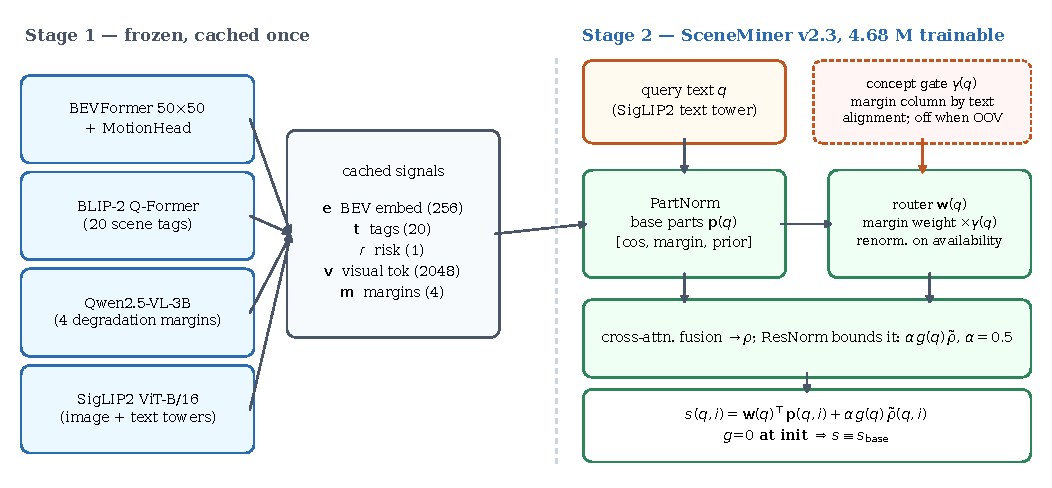
\includegraphics[width=\textwidth]{figures/fig1_architecture.pdf}
\caption{\textbf{SceneMiner.} Stage~1 is frozen and cached once per scene.
Stage~2 ($4.68$M trainable parameters) standardises three base parts
(\textsc{PartNorm}), routes them per query, and adds a cross-attention residual
that \textsc{ResNorm} standardises and bounds. A factored concept gate, built
only from training phrasings, gives $\gdeg(q)$ (does a degradation concept
apply?) and $\gmac(q)$ (which recorded context does the query name?). The score
trusts the learned head in proportion to $\gdeg$ and otherwise abstains to
SigLIP2 plus the metadata named by $\gmac$. Monocular mode masks the 3D tokens.}
\label{fig:arch}
\end{figure*}

% =====================================================================
\section{Related work}
% =====================================================================

\paragraph{Driving data and language.} nuScenes~\cite{caesar2020nuscenes},
Waymo Open~\cite{sun2020waymo} and BDD100K~\cite{yu2020bdd} supply the scenes we
mine and test on; adverse-condition benchmarks such as
ACDC~\cite{sakaridis2021acdc} pair degraded and clear views for segmentation.

\paragraph{Driving scene retrieval.} BEV-TSR~\cite{tang2025bevtsr} aligns text
with multi-camera BEV features for text-to-scene retrieval.
CARIM~\cite{ki2025carim} captions scenes with a VLM and retrieves by inclusive
text matching. RefAV~\cite{davidson2025refav} mines scenarios by having an LLM
compile the query into a program over tracked 3D objects, and
ReferGPT~\cite{chamiti2025refergpt} matches text descriptions of tracked objects'
3D state to a referring expression with CLIP. Talk2BEV~\cite{choudhary2024talk2bev}
and nuPrompt~\cite{wu2023nuprompt} attach language to BEV maps and to objects; we
use nuPrompt-style tags as a Stage-1 signal and show that this contaminates
semantic evaluation on the same scenes. Each of these systems reads one signal
family, and their releases need inputs our corpora lack (tracks, HD maps, an
LLM service). We therefore re-implement each \emph{paradigm} on our cached
signals (\cref{sec:results}); the comparison is between paradigms, not the
published systems.

\paragraph{Vision--language retrieval.} Contrastive image--text models,
CLIP~\cite{radford2021clip} and the sigmoid-loss
SigLIP~\cite{zhai2023siglip,tschannen2025siglip2}, give zero-shot retrieval;
BLIP-2~\cite{li2023blip2} and Qwen2.5-VL~\cite{bai2025qwen25vl} answer attribute
questions whose yes/no log-odds we use as margins. Our strongest external
baseline is frozen SigLIP2, and our strongest conjunction baseline adds recorded
metadata to it.

\paragraph{Shortcuts, routing and normalisation.} Models that lean on the
easiest predictive signal are a known failure mode~\cite{geirhos2020shortcut};
gated mixtures collapse onto few experts without balancing
pressure~\cite{shazeer2017moe}. Balancing the router is not enough when the
routed quantities are on different scales; the remedy is the running
standardisation familiar from batch normalisation~\cite{ioffe2015bn}.
Contrastive text embeddings are anisotropic, and mean removal restores
discriminative similarity~\cite{mu2018allbutthetop,ethayarajh2019anisotropy}.

\paragraph{Evaluation.} We correct for multiple comparisons with
Benjamini--Hochberg~\cite{benjamini1995fdr}, use spectral effective
rank~\cite{roy2007erank} in diagnostics, and MMR-style
diversity~\cite{carbonell1998mmr} for top-$k$ composition.

% =====================================================================
\section{Setup}
% =====================================================================

\paragraph{Corpus and splits.} $1508$ scenes from nuScenes and Waymo, split
\emph{segment-disjoint} into $906$ training scenes ($422$ nuScenes, $484$ Waymo;
$121$ segments) and $602$ evaluation scenes ($278$, $324$; $81$ segments). No
evaluated scene contributes a gradient. All $700$ nuScenes corpus scenes belong
to the official nuScenes \emph{train} split; the $150$ official \emph{val}
scenes form a separate, uncontaminated set (\emph{val150}).

\paragraph{Stage 1 (frozen).} BEVFormer~\cite{li2022bevformer} with a
$50\times50$ grid and a motion head gives a $256$-d embedding $\mathbf{e}$ and a
risk scalar $r$; a BLIP-2 Q-Former gives $20$ tag logits $\mathbf{t}$;
Qwen2.5-VL-3B gives a $2048$-d visual token $\mathbf{v}$ and four margins
$\mathbf{m}$ (droplets, glare, wet road, low contrast), each the yes--no log-odds
of a fixed question; SigLIP2 ViT-B/16 gives aligned image and text embeddings. A
$26$-d prior $\pi$ holds the $20$ tags and six one-hots of recorded metadata
(night, day, rain, dry, dense, sparse).

\paragraph{Queries.} $390$ queries ($240$ train, $150$ evaluation) in four
strata: sensor degradation (S1, $62$), macro-environmental (S2, $58$),
compositional held-out (S3, $18$) and negated (S4, $12$). A fifth stratum of
$40$ semantic edge-case queries is introduced in \cref{sec:regimes}.

\paragraph{Human ground truth.} One rater labelled $600$ evaluation scenes for
the four degradation attributes; $550$ remain after removing $50$ scenes the
rater marked unsure and left unlabelled. Stratum~5 additionally uses nuScenes
human 3D annotation and human-written scene descriptions. No human label enters
training.

% =====================================================================
\section{The benchmark is circular}
\label{sec:d1}
% =====================================================================

The standard suite marks a scene relevant when it satisfies a predicate over
cached attributes, \eg $\{\texttt{droplets}{=}\texttt{true}\}$ or
$\{\texttt{lighting}{=}\texttt{night}\}$. Those attributes are the Stage-1 VLM's
own outputs and recorded metadata, so an index reading them scores $1.000$~mAP,
$0.992$~P@5 and $1.000$~NDCG@10 on the $150$ evaluation queries
(\cref{fig:audit}a). That is the benchmark restating its definition: every
learned number is measured against an unreachable ceiling, and any method moving
\emph{toward} the cached decisions scores better whether or not they are right.
Often they are not: against $550$ human-labelled scenes, the VLM's precision on
its own four attributes is $0.50$--$0.68$. We therefore report the index as a
ceiling and give evidential weight to human labels, an external corpus and human
3D annotation.

% =====================================================================
\section{The certifiers are contaminated}
\label{sec:d2}
% =====================================================================

Mining is justified by a downstream claim, that the mined scenes are hard for
the perception stack. Testing that needs a detector that has not memorised them.
\texttt{bevformer\_base} ($0.4164$~mAP / $0.5173$~NDS globally, reproducing the
checkpoint), evaluated per scene with the official nuScenes
\texttt{accumulate}/\texttt{calc\_ap},\footnote{A class-agnostic per-scene
matcher inverts the signal, scoring night scenes $150\times$ higher than day.
Under the official protocol night is $0.4171$ and day $0.4553$.} scores $0.7864$
on the $278$ corpus scenes from its training split and $0.4514$ on the $150$ val
scenes it never saw: $+0.3349$~mAP ($+74\%$) of memorisation
(\cref{fig:audit}b). The tag head is contaminated too: it was supervised with
nuPrompt-style tags for all $850$ nuScenes scenes, which include
\texttt{object\_pedestrian}, \texttt{object\_bus} and
\texttt{scene\_construction\_zone}. Every downstream claim below uses val150,
and any ranker reading $\mathbf{e}$, $r$ or $\mathbf{t}$ on corpus scenes is
marked\cont.

\begin{figure*}[t]
\centering
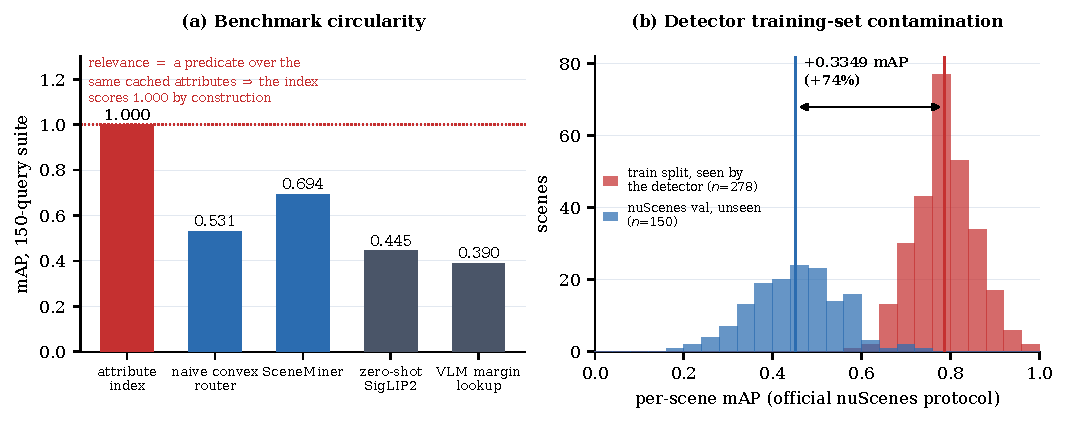
\includegraphics[width=\textwidth]{figures/fig3_audit.pdf}
\caption{\textbf{Two structural defects.} (a) Relevance is a predicate over the
same cached attributes an index can read, so the index scores $1.000$ by
construction; the naive convex router and SceneMiner are measured against that
ceiling. (b) The certifying detector scores $+0.3349$~mAP higher on scenes it
was trained on than on unseen validation scenes.}
\label{fig:audit}
\end{figure*}

% =====================================================================
\section{Silent modality failure in learned fusion}
\label{sec:d3}
% =====================================================================

The natural fusion design combines a SigLIP2 cosine, a selected VLM margin and a
metadata prior with query-conditioned convex weights $\mathbf{w}(q)$, plus a
gated cross-attention residual. Trained on VLM pseudo-labels, this \emph{naive
convex router} puts $0.967$--$0.992$ of its weight on the margin, a teacher
shortcut, and scores $0.486$ on BDD100K against $0.622$ for zero-shot SigLIP2.
Repairing the router alone (channel dropout, an entropy floor, modality masking)
lowers the margin weight from $0.980$ to $0.535$ but moves external mAP by
$-0.001$. Three scale defects are the cause, and none shows in task mAP.

\paragraph{Level 1: the parts.} The blend scores \emph{below both signals it
blends} ($0.485$ vs.\ $0.622$ and $0.587$), which no convex combination of
commensurate signals can do: the margin part has $30.3\times$ the spread of the
cosine (std $0.583$ vs.\ $0.019$), so a nominal $50/50$ weight is $\sim\!97\%$
margin. Running training stds show it without labels: $[0.031, 0.566, 0.159]$.

\paragraph{Level 2: the residual} has $2$--$3\times$ the spread of the base it
corrects (training std $6.31$ against $0.03$--$0.57$): the routed base alone
scores $0.9609$ on droplets, $0.8813$ with the residual.

\paragraph{Level 3: a dead modality.} LayerNorm over a width-1 scalar returns
$(x-\bar x)/\sqrt{0+\epsilon}\equiv0$, so a fusion head that LayerNorms each
modality gives the risk token \emph{one} value across all $1508$ scenes. Task mAP
does not notice: $0.311\pm0.036$ with the dead token, $0.307\pm0.048$ with it
restored by scalar standardisation (five seeds, predicate suite).

\begin{quote}\itshape
A fusion weight is an influence weight only if what it weighs is standardised,
at every level at which signals are combined. Task mAP will not tell you when
it is not.
\end{quote}

% =====================================================================
\section{SceneMiner}
\label{sec:method}
% =====================================================================

For query $q$ and scene $i$ (arguments $(q,i)$ omitted), with standardised parts $\tilde{\mathbf{p}}$,
\begin{align}
s_{\mathrm{head}} &= \mathbf{w}(q)^{\!\top}\tilde{\mathbf{p}}+\alpha\,g(q)\,\tilde\rho,\nonumber\\
s &= \gdeg(q)\,s_{\mathrm{head}}+\big(1-\gdeg(q)\big)\,s_{\mathrm{abst}}.
\label{eq:score}
\end{align}
Scoring all $1508$ scenes for one query takes $7.93\pm0.20$\,ms on an A40.

\paragraph{\textsc{PartNorm} and \textsc{ResNorm}.} The parts
$[\cos, m_{\mathrm{sel}}, \pi_{\mathrm{sel}}]$ and the residual $\rho$ are
standardised by running statistics computed on the $906$ training scenes and
frozen at inference; scalar inputs are standardised, never LayerNormed. The
residual enters bounded, $|g|\le1$, $\alpha=0.5$, so it corrects the base by at
most half a part standard deviation.

\paragraph{A concept bank from training text.} Only four margin columns exist, so
the model must decide per query whether one applies. We build $23$ classes from
\emph{training text only}: four concept classes from the $156$ sensor-degradation
phrasings of the $390$-query training split, seven context classes from its $84$
macro-environmental phrasings grouped by predicate (night, day, rain, dry, dense,
sparse, moderate), and $12$ generic phrases. Embeddings are mean-centred with the
bank's own mean, because SigLIP2's text space is anisotropic and raw
text--text cosine does not separate the bank. Each class scores a query by a soft
maximum, $S_k(q)=\tau\log\frac{1}{|k|}\sum_{i\in k}\exp(\cos(q,b_i)/\tau)$.

\paragraph{A factored gate.} Degradation and context are independent axes:
``slick pavement in the dark'' names both. A single softmax over all $23$ classes
makes them compete, and the context class steals the concept's mass. We
therefore factor the gate.
\begin{itemize}\setlength{\itemsep}{0pt}
\item $\gdeg(q)=\sum_{k\in\text{concepts}}\mathrm{softmax}_k(S'(q)/\tau)$, where
  $S'$ is computed after removing half of the context subspace (the span of the
  seven context-class means) from query and bank. A context word then no longer
  pulls a degradation query toward a foil.
\item $\gmac(q)$: the unprojected softmax mass $\gamma_m$ on each context class
  $m$ that has a recorded-metadata column.
\end{itemize}
The abstention target adds the metadata the query names, standardised with
training-scene statistics,
\begin{equation}
s_{\mathrm{abst}}=\Big(\tilde p_{\cos}+\textstyle\sum_m\gamma_m z_m\Big)\Big/\sqrt{1+\big(\textstyle\sum_m\gamma_m\big)^2},
\label{eq:abst}
\end{equation}
and reduces to the SigLIP2 cosine where no metadata exists (BDD100K). The margin
column is $\mathrm{softmax}(S'_{\text{concepts}}/0.1)$, and the margin's routing
weight is multiplied by $\gdeg$.

\paragraph{Choosing the gate on training text.} Projection strength and $\tau$
are selected without any evaluation query (grid in the supplementary): positives
are the $156$ degradation phrasings, scored leave-group-out (a base phrasing and
all its compounds held out together); negatives are the $96$ context and generic
phrasings and $60$ synthetic context$\times$context conjunctions. Maximising the
share of positives with $\gdeg>0.9$ while every negative stays $\le0.2$ selects
half projection and $\tau=0.02$.

\paragraph{False-negative rescue.} When $\tilde p_{\cos}>1$, the standardised
margin is lower-clamped at $-0.5$, so a confident VLM ``no'' cannot veto a strong
visual match.

\paragraph{Training.} Channel dropout ($50\%$ of steps drop the margin, $30\%$ the
3D tokens), an entropy floor on routing, and pair weights from agreement between
the two frozen teachers; listwise InfoNCE plus a conditional hinge, $3000$ AdamW
steps, five seeds of under a minute each on one A40. Gate and selectors start at
zero, so $s_{\mathrm{head}}\equiv$ base at step~$0$ (full settings in the
supplementary).

% =====================================================================
\section{Results}
\label{sec:results}
% =====================================================================

\begin{table}[t]\centering\small
\caption{\textbf{Design progression}, each row trained with the same recipe.
Human GT: macro-mAP on $550$ scenes, zero-leakage / calibrated (routing weights
refit on $4/5$ of the scenes, scored on the held-out $1/5$). Suite: $150$-query mAP
and top-5 domain skew.}
\label{tab:design}
\resizebox{\columnwidth}{!}{%
\begin{tabular}{lccc}
\toprule
design & human GT & BDD100K & suite / skew\\
\midrule
naive convex router & $0.736$ / $0.792$ & $0.486$ & $0.531$ / $+8.7$\\
$+$ anti-collapse routing, \textsc{PartNorm} & $0.707$ / $0.766$ & $0.570$ & $0.518$ / $+1.1$\\
$+$ \textsc{ResNorm}, single-prompt gate & \best{0.790} / \best{0.828} & $0.589$ & $0.631$ / $+17.0$\\
$+$ contrastive gate, abstention & $0.788$ / $0.817$ & \best{0.628} & $0.594$ / \best{$+0.5$}\\
\textbf{SceneMiner} (factored gate) & $0.785$ / $0.826$ & $0.616$ & \best{0.685} / $+2.2$\\
\bottomrule
\end{tabular}%
}
\end{table}

\paragraph{Design progression.} \cref{tab:design}. Each step fixes one named
defect. Routing repair alone moves BDD100K by $-0.001$ (\cref{sec:d3}); adding
\textsc{PartNorm} raises it by $+0.084$ at an in-domain cost; \textsc{ResNorm}
gives the largest in-domain gain; the contrastive gate and abstention give the
first external result above SigLIP2 and remove the domain skew; and the factored
gate recovers compositional queries. No single design wins every column.
SceneMiner trades $0.012$ BDD100K mAP against the unfactored gate for $+0.091$ on
the suite; most of the difference is one query, ``snow covering the road'', whose
$\gdeg$ rises from $0.49$ to $0.71$ once the context subspace is removed
(per-query table in the supplementary).

\begin{table*}[t]\centering\small
\caption{\textbf{SceneMiner against published driving-retrieval paradigms and
foundation models}, identical splits, queries and metrics (mAP). Rows marked
``-style'' re-implement the paradigm on our cached signals (specified in the supplementary);
they are not the authors' systems. Stratum~5: $40$ semantic queries graded by
human 3D annotation on $258$ corpus scenes, and the subset with $\ge3$ positives
on the uncontaminated val150. ms: online ranking of $1508$ cached scenes, one
model, A40, excluding query encoding. n/a: the method needs a signal the corpus
lacks (BEV and tags on monocular images). \cont~reads the BEV embedding or tags,
which were supervised on corpus scenes. $^{\ddagger}$reads the very attributes
that define suite relevance (\cref{sec:d1}).}
\label{tab:master}
\setlength{\tabcolsep}{3.5pt}
\begin{tabular}{llcccccccc}
\toprule
 & & human GT & \multicolumn{2}{c}{BDD100K} & \multicolumn{2}{c}{Stratum 5} & \multicolumn{2}{c}{150Q suite} & ms\\
\cmidrule(lr){4-5}\cmidrule(lr){6-7}\cmidrule(lr){8-9}
method & modalities & ($550$) & $1000$ & holdout & $258$ & val150 & mAP & skew & ($1508$)\\
\midrule
BEV-TSR-style~\cite{tang2025bevtsr} & BEV & 0.577\cont & n/a & n/a & 0.208\cont & n/a & 0.459\cont & $+26.5$ & $0.39$\\
RefAV-style (LLM program)~\cite{davidson2025refav} & VLM flags, tags, meta & 0.717\cont & 0.432 & 0.184 & 0.188\cont & 0.198 & 0.823\cont$^{\ddagger}$ & $+5.1$ & $0.06$\\
CARIM-style (neutral captions)~\cite{ki2025carim} & VLM captions & 0.274 & 0.440 & 0.293 & 0.227 & 0.320 & 0.268 & $+0.3$ & $1.05$\\
CARIM-style (listing captions)~\cite{ki2025carim} & VLM captions & 0.377 & 0.463 & n/a & 0.248 & 0.309 & 0.308 & $-5.9$ & $1.53$\\
Tag map~\cite{choudhary2024talk2bev,wu2023nuprompt} & BEV tags & 0.624\cont & n/a & n/a & 0.198\cont & n/a & 0.378\cont & $+28.6$ & $0.67$\\
ReferGPT-style~\cite{chamiti2025refergpt} & image, tags, meta & 0.469\cont & 0.612 & 0.353 & 0.252\cont & 0.376 & 0.543\cont & $+3.8$ & $1.40$\\
\midrule
CLIP ViT-B/32~\cite{radford2021clip} & image & 0.453 & 0.612 & 0.353 & 0.253 & 0.374 & 0.384 & $-11.7$ & $0.17$\\
SigLIP ViT-B/16~\cite{zhai2023siglip} & image & 0.507 & 0.607 & 0.388 & 0.281 & 0.385 & 0.427 & $-12.9$ & $0.17$\\
SigLIP2 ViT-B/16~\cite{tschannen2025siglip2} & image & 0.569 & \best{0.622} & \best{0.408} & \best{0.312} & 0.385 & 0.445 & $-16.2$ & $0.17$\\
SigLIP2 + adapter (906 scenes) & image & 0.666 & 0.539 & 0.239 & 0.222 & 0.226 & 0.479 & $-7.3$ & $0.39$\\
Qwen2.5-VL lookup~\cite{bai2025qwen25vl} & VLM margins & 0.732 & 0.587 & 0.231 & 0.219 & 0.231 & 0.414$^{\ddagger}$ & $-10.1$ & $0.01$\\
\midrule
Naive convex router & all & 0.735\cont & 0.486 & 0.215 & 0.188\cont & 0.212 & 0.531\cont & $+8.7$ & $5.81$\\
\textbf{SceneMiner} (portable) & image, VLM, meta & 0.762 & 0.614 & 0.400 & 0.311 & \best{0.394} & 0.654 & $-13.9$ & $2.47$\\
\textbf{SceneMiner} (full) & all & \best{0.794}\cont & 0.614 & 0.400 & 0.308 & \best{0.394} & \best{0.694}\cont & $+2.6$ & $3.51$\\
\bottomrule
\end{tabular}

\end{table*}

\paragraph{Against published paradigms.} \cref{tab:master}. On human-labelled
degradation SceneMiner leads all eleven alternatives ($0.785$; next the naive
router $0.735$, the RefAV-style program $0.733$ and the lookup $0.732$). Each
single-family paradigm fails somewhere. BEV-only retrieval and the tag map cannot
run on monocular images, and on Stratum~5 they stay near the lookup's chance level
even on the scenes their encoders were trained on. The RefAV-style program scores
$0.850$ on the suite because its predicates \emph{are} the suite's relevance
attributes, then falls to $0.383$ on BDD100K, where they are not. Caption matching
is weak on degradations because captions mention a degradation mostly to deny it
($64\%$ of captions say there are no droplets or glare). Fine-tuning SigLIP2 on our
$906$ training scenes lifts human GT to $0.666$ but costs $0.083$ on BDD100K and
$0.09$--$0.16$ on Stratum~5. SigLIP2 stays the strongest single model on BDD100K ($0.622$
vs.\ $0.616$, $p=0.94$) and ties SceneMiner on Stratum~5 ($p\ge0.33$). On the $4$
val150 conjunctions CLIP and the ReferGPT-style ranker score higher ($0.65$,
$0.69$ vs.\ $0.42$), too few queries to test. Ranking is under $8$\,ms for every
method; the caption baseline additionally needs $3.6$\,s of VLM decoding per
image offline.

\begin{table}[t]\centering\small
\caption{\textbf{Ablations of SceneMiner}, one inference switch each.}
\label{tab:abl}
\resizebox{\columnwidth}{!}{%
\begin{tabular}{lccc}
\toprule
variant & human GT & BDD100K & suite / skew\\
\midrule
\textbf{SceneMiner} & \best{0.7845} & \best{0.6164} & \best{0.685} / $+2.2$\\
without metadata in $s_{\mathrm{abst}}$ & \best{0.7845} & -- & $0.606$ / $-0.2$\\
without abstention & \best{0.7845} & $0.6074$ & $0.634$ / $+17.0$\\
without $\gdeg$ on routing & \best{0.7845} & $0.6138$ & \best{0.685} / $+2.1$\\
without \textsc{ResNorm} & $0.7689$ & -- & $0.633$ / $+2.2$\\
\bottomrule
\end{tabular}%
}
\end{table}

\paragraph{Human ground truth.} SceneMiner scores $0.7845$ zero-leakage and
$0.8263$ calibrated, against $0.7372$ for the strongest no-learning control (late
fusion of SigLIP2 with the lookup). Per attribute: $0.9443$ (droplets), $0.5750$
(glare), $0.9725$ (wet road), $0.6463$ (low contrast). All four canonical queries
have $\gdeg=1.000$, so the gate and abstention change nothing here
(\cref{tab:abl}); \textsc{ResNorm} is worth $0.016$, and without it recovery of
VLM-missed glare scenes falls from $7/20$ to $4/20$.

\begin{table}[t]\centering\small
\caption{\textbf{External transfer}, BDD100K: $1000$ images, $12$ queries,
native human labels, chance $0.262$. In-vocabulary: the $4$ queries naming a
cached attribute (fixed from wording). BDD100K has no metadata, so
$s_{\mathrm{abst}}$ is the SigLIP2 cosine. No tuning on BDD100K.}
\label{tab:bdd}
\resizebox{\columnwidth}{!}{%
\begin{tabular}{lccccc}
\toprule
ranker & all & in-voc & OOV & P@5 & NDCG@10\\
\midrule
\textbf{SceneMiner} & $0.6164$ & \best{0.7003} & $0.5745$ & $0.817$ & $0.782$\\
zero-shot SigLIP2 & \best{0.6218} & $0.6002$ & \best{0.6327} & \best{0.850} & \best{0.809}\\
logit VLM lookup & $0.5871$ & $0.6475$ & $0.5569$ & $0.717$ & $0.705$\\
\bottomrule
\end{tabular}%
}
\end{table}

\paragraph{External transfer.} \cref{tab:bdd} (per query in the supplementary). SceneMiner is
$0.005$ below zero-shot SigLIP2 overall ($0.6164$ vs.\ $0.6218$): it gains $+0.100$
on in-vocabulary queries and loses $0.058$ out of vocabulary. The gate switches off context and weather queries that a single-prompt
gate mistakes for degradation (``bright daytime driving'', ``driving after dark'':
$\gdeg=0.000$). Two out-of-vocabulary queries still trigger it, ``overcast grey
sky'' (as low contrast) and ``snow covering the road'' (as wet road), and they
account for the OOV gap. No training phrasing describes overcast skies or snow;
adding such foils would tune the gate on BDD100K, so we did not.

\begin{figure*}[t]
\centering
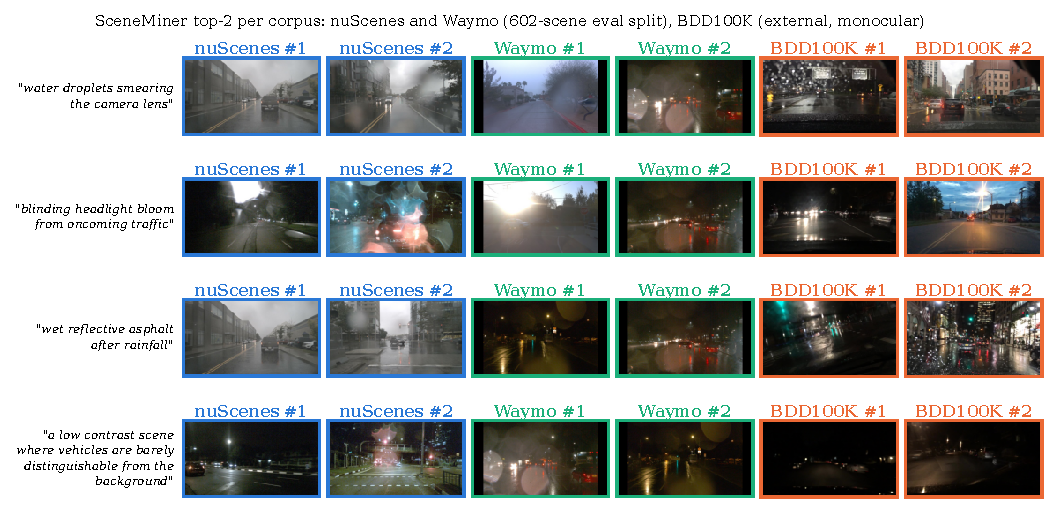
\includegraphics[width=0.9\textwidth]{figures/fig2_qualitative.pdf}
\caption{\textbf{Qualitative retrievals, balanced across corpora}: SceneMiner's
top two within each of nuScenes and Waymo (evaluation split, one per driving
segment) and BDD100K (external, portable signals). (a) Sensor and surface
degradations. (b) Safety-critical road users and objects; yellow boxes are human
3D annotations of the queried class projected into the retrieved frame, the inset
enlarges the smallest, and red labels mark retrievals with none. Waymo's labels
lack truck, bus and cone classes; BDD100K boxes are not available.}
\label{fig:qual}
\end{figure*}

\begin{table}[t]\centering\small
\caption{\textbf{150-query suite} by stratum, $602$ evaluation scenes. Relevance
is cached attributes and metadata (\cref{sec:d1}); the index is a ceiling.}
\label{tab:suite}
\resizebox{\columnwidth}{!}{%
\begin{tabular}{lcccccc}
\toprule
ranker & S1 & S2 & S3 & S4 & all & skew\\
\midrule
attribute index (ceiling) & $1.00$ & $1.00$ & $1.00$ & $1.00$ & $1.000$ & --\\
\textbf{SceneMiner} & $0.755$ & \best{0.671} & $0.603$ & \best{0.511} & \best{0.685} & $+2.2$\\
\enspace without metadata in $s_{\mathrm{abst}}$ & $0.754$ & $0.487$ & $0.543$ & $0.508$ & $0.606$ & $-0.2$\\
\enspace without abstention & $0.755$ & $0.520$ & \best{0.689} & $0.482$ & $0.634$ & $+17.0$\\
zero-shot SigLIP2 & $0.444$ & $0.487$ & $0.370$ & $0.355$ & $0.445$ & $-16.2$\\
logit VLM lookup & $0.586$ & $0.270$ & $0.052$ & $0.467$ & $0.390$ & $-6.6$\\
\bottomrule
\end{tabular}%
}
\end{table}

\paragraph{150-query suite.} \cref{tab:suite}. Overall mAP rises to $0.685$ with
skew $+2.2$ points (CI $[-2.6,+6.8]$). Two caveats apply. The S2 gain
($0.487\rightarrow0.671$) is partly circular: S2 relevance \emph{is} recorded
metadata, which $s_{\mathrm{abst}}$ now reads. S3 recovers from $0.459$ (single
softmax gate) to $0.603$ but stays below the $0.689$ of the un-gated head. Its
context$\times$context queries (``heavy rain at night'') are served by metadata;
some degradation$\times$context compounds are still gated off.

% =====================================================================
\section{Where learned fusion helps, and where it does not}
\label{sec:regimes}
% =====================================================================

\paragraph{Stratum 5: semantic edge cases.} From official nuScenes human 3D
annotation in the CAM\_FRONT field of view (visibility $>40\%$, in $\ge25\%$ of
keyframes) we derive five scene flags: pedestrian within $25$\,m; vulnerable road
user (VRU); construction zone; bus, truck or trailer within $25$\,m; rare
categories (child, stroller, wheelchair, police, emergency vehicle, debris).
Night and rain come from the human scene description. $20$ atomic queries and $20$
conjunction phrasings cover the $12$ cells with $\ge5$ positives among the $258$
human-labelled evaluation scenes (definitions in the supplementary).

\begin{table}[t]\centering\small
\caption{\textbf{Three human-graded regimes}, mAP. Late fusion adds $z$-scored
rankers with no learning. On object queries the lookup and metadata are constant
(chance), so both fusions reduce to SigLIP2. SceneMiner rows score the 5-seed
ensemble ($0.789$); \cref{tab:design,tab:abl,tab:master} average per-seed mAP ($0.785$).}
\label{tab:regimes}
\resizebox{\columnwidth}{!}{%
\begin{tabular}{lccc}
\toprule
ranker & degradation & semantics & sem.$\times$cond.\\
 & ($550$) & ($258$ / val150) & ($258$)\\
\midrule
\textbf{SceneMiner} & \best{0.789} & $0.332$ / \best{0.392} & $0.310$\\
zero-shot SigLIP2 & $0.569$ & \best{0.337} / $0.382$ & $0.293$\\
logit VLM lookup & $0.733$ & $0.217$ / $0.220$ & $0.227$\\
fusion SigLIP2 $+$ lookup & $0.737$ & $=$ SigLIP2 & $0.284$\\
fusion SigLIP2 $+$ metadata & $0.626$ & $=$ SigLIP2 & \best{0.327}\\
\bottomrule
\end{tabular}%
}
\end{table}

\paragraph{Three regimes.} \cref{tab:regimes,fig:loop}b. On \emph{atomic
degradation}, the regime it was trained for, SceneMiner leads the strongest
no-learning control by $+0.052$. On \emph{atomic semantics} the lookup and
metadata are at chance and every sensible ranker reduces to SigLIP2; object
queries get $\gdeg\approx0$, so SceneMiner abstains and matches it ($-0.005$,
$p=0.42$; val150 $+0.010$, $p=0.33$; $+0.115$ over the lookup, $p=0.0001$). On
\emph{object$\times$condition conjunctions} it beats SigLIP2 ($+0.016$, $p=0.33$)
and the lookup ($+0.080$, $p=0.044$) through the metadata in $s_{\mathrm{abst}}$,
but the no-learning fusion of SigLIP2 with that metadata is higher ($-0.017$,
$p=0.17$). For night and rain that metadata is the scene description that defines
the ground truth, so this control is the right bar. Rare categories are at chance
for every ranker, and a tag readout supervised on these scenes\cont{} beats
SigLIP2 only on heavy vehicles ($0.392$).

\paragraph{A simulated second rater.} Tables in the supplementary. We have one
rater. Its $50$ unsure scenes carry no labels, so they cannot be scored. Removing
the scenes CLIP finds most ambiguous \emph{widens} SceneMiner's lead over the
lookup ($+0.056\rightarrow+0.089$). A Monte Carlo second rater at $\kappa$ of $0.90$,
$0.85$ and $0.75$ keeps SceneMiner ahead of SigLIP2 in every trial and ahead of
the lookup in $92$--$100\%$. The lead is not uniform: it rests on low contrast and
droplets, glare and wet road are near coin flips against the lookup, and glare is
lost to late fusion in nearly every trial. The macro claim is robust; a
per-attribute claim would be overstated.

% =====================================================================
\section{Does the premise hold?}
\label{sec:premise}
% =====================================================================

\paragraph{Degradation damages detection, in the right sector.} A whole-scene
test finds nothing ($<0.07\sigma$): it averages mAP over six cameras and
$360^\circ$ while the degradation signal comes from one camera, and only
$23.4\%$ of nuScenes ground truth lies in the CAM\_FRONT field of view. Measuring
degradation and error in the same sector on val150 (\cref{tab:premise}; official
\texttt{accumulate}/\texttt{calc\_ap}/\texttt{calc\_tp}; greedy $2$\,m matching at
score $0.3$ for FP rate and recall; scene bootstrap; permutation tests;
Benjamini--Hochberg over $30$ tests), degraded front cameras cost $9.1$ points of
front-sector mAP and raise the false-positive rate at the mining operating point
by $7.3$ points ($+26\%$ relative). Four of the $30$ tests survive at $q<0.05$ and
$12$ at $q<0.10$. Orientation error does not move. Lens degradations hit mAP
hardest; low contrast hits far recall hardest ($-0.0973$). With $6$ degraded
scenes, glare is underpowered rather than null.

\begin{table}[t]\centering\small
\caption{\textbf{CAM\_FRONT degradation vs.\ 3D error}, val150, $42$ degraded
vs.\ $108$ clean scenes, front sector only; $q$: Benjamini--Hochberg.}
\label{tab:premise}
\begin{tabular}{lccrc}
\toprule
metric & degraded & clean & $\Delta$ & $q$\\
\midrule
mAP & $0.3886$ & $0.4792$ & $-0.0906$ & \best{0.015}\\
ghost FP @ $s{>}0.3$ & $0.3503$ & $0.2775$ & $+0.0729$ & \best{0.045}\\
mATE (m) & $0.8330$ & $0.7553$ & $+0.0777$ & $0.080$\\
recall $>30$\,m & $0.5312$ & $0.6079$ & $-0.0767$ & $0.080$\\
mAOE (rad) & $0.5008$ & $0.4308$ & $+0.0701$ & $0.489$\\
\bottomrule
\end{tabular}
\end{table}

\begin{table}[t]\centering\small
\caption{\textbf{Retrieval to breakage}, val150, $62$ degradation queries:
top-$25$ front-sector metric minus the val150 mean. $^{*}p<0.05$, one-sided,
scene-permutation null with retrieved sets fixed.}
\label{tab:loop}
\resizebox{\columnwidth}{!}{%
\setlength{\tabcolsep}{4pt}
\begin{tabular}{lcccc}
\toprule
ranker & mAP & ghost FP & rec.\,$>30$\,m & VRU rec.\\
\midrule
\textbf{SceneMiner} & $-0.056$$^{*}$ & $+0.024$ & $-0.040$ & $-0.197$$^{*}$\\
VLM margin lookup & $-0.054$$^{*}$ & $+0.026$ & $-0.041$ & $-0.191$$^{*}$\\
night/rain metadata & $-0.066$$^{*}$ & $+0.052$$^{*}$ & $-0.055$$^{*}$ & $-0.167$$^{*}$\\
zero-shot SigLIP2 & $-0.032$$^{*}$ & $+0.019$ & $-0.027$ & $-0.098$$^{*}$\\
random & $+0.000$ & $+0.001$ & $+0.001$ & $-0.000$\\
\bottomrule
\end{tabular}
%
}
\end{table}

\begin{figure*}[t]
\centering
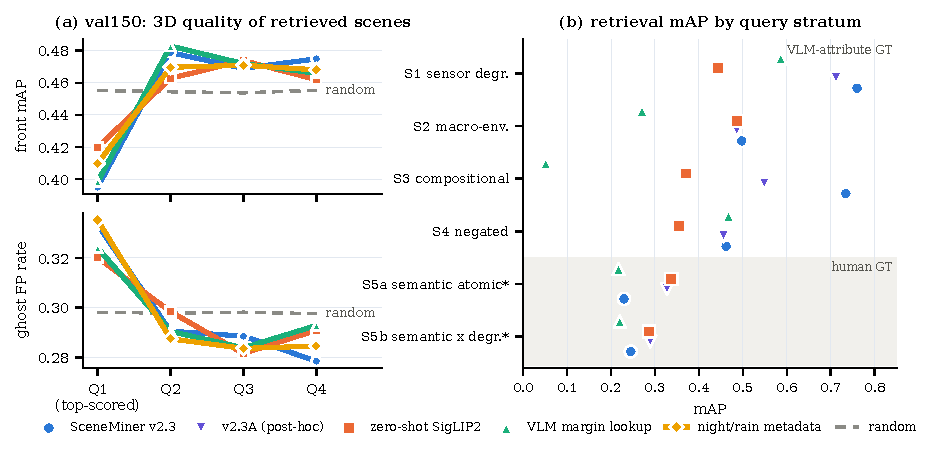
\includegraphics[width=0.85\textwidth]{figures/fig4_front_sector_degradation_and_semantics.pdf}
\caption{\textbf{(a)} On uncontaminated val150, the top-scored quartile of the
$62$ degradation queries has lower CAM\_FRONT mAP and a higher ghost-FP rate for
every informative ranker; Q2--Q4 sit at the corpus mean. \textbf{(b)} mAP in the
three human-graded regimes against two no-learning fusion controls.}
\label{fig:loop}
\end{figure*}

\paragraph{From retrieval to breakage.} Every ranker scores val150 from
portable signals (SigLIP2 on the CAM\_FRONT keyframe, CAM\_FRONT margins, and the
recorded night/rain metadata), and we read the detector's front-sector metrics on
what it retrieved. Similar queries retrieve overlapping scenes, so the null
permutes per-scene metrics while each retrieved set stays fixed. SceneMiner's
top-$25$ loses $0.057$ mAP ($p=0.002$) and $0.197$ vulnerable-road-user recall
($-0.80\sigma$, $p<0.001$; \cref{tab:loop}), and is significantly harder than
SigLIP2's (mAP $-0.025$, $p=0.014$; VRU recall $-0.099$, $p<0.001$). It is
indistinguishable from the VLM-margin lookup on every metric, and night/rain
metadata retrieves scenes with significantly more ghost false positives than
SceneMiner's ($+0.028$, $p=0.030$). The effect is a threshold confined to the top
quartile (\cref{fig:loop}a). For semantic queries, retrieving the requested
objects does not find harder scenes: pedestrians, cones and trucks are not
harder for this detector than anything else.

% =====================================================================
\section{Discussion}
% =====================================================================

\paragraph{What we claim.} Front-camera degradation measurably breaks 3D detection
on uncontaminated data, and language-guided retrieval surfaces a top quartile
where it does. Benchmarks defined as predicates over cached outputs cannot
measure progress, and certifiers trained on the mined scenes cannot certify them.
A learned fusion must standardise what it combines at every level, because task
mAP will not reveal a dead or dominating modality. It must also know when its
training vocabulary applies, and abstain when it does not.

\paragraph{What we do not claim.} That learned fusion beats a no-learning fusion
of SigLIP2 with metadata on object$\times$condition conjunctions: it does not. That
SceneMiner finds breakage scenes better than the VLM-margin lookup on val150: it
does not. That its in-domain lead is uniform: glare and wet road are near ties
with the lookup. That it beats every paradigm everywhere: SigLIP2 ties it on
BDD100K and Stratum~5 (\cref{tab:master}).

\paragraph{Limitations.} One human rater; four degradation attributes; one
monocular external corpus; Stratum-5 conjunctions with $5$--$12$ positives; val150
scored only from portable signals. Three components, text mean-centring,
\textsc{ResNorm} and the gate factorisation, were identified while diagnosing
failures on evaluation data. None has a parameter fitted to evaluation data, and
each is supported by training-only evidence (\cref{sec:d3,sec:method}).

\paragraph{For the community.} Four cheap checks catch every defect here: score a
lookup over your own cached labels; ask whether the certifier trained on your
corpus; inspect the scales of what a fusion combines; and measure an effect where
its cause acts. Code, data and all result files will be released.

{
    \small
    \bibliographystyle{ieeenat_fullname}
    \bibliography{main}
}

\end{document}
